\documentclass[12pt]{report}
\usepackage[a4paper, total={7.3in, 9.7in}]{geometry}
\usepackage{amsmath}
\usepackage{upquote}
\usepackage{listings}
\usepackage{xcolor}
\usepackage{titlesec}
\usepackage{amssymb}

\definecolor{backgroundcolor}{rgb}{1, 1, 1}
\definecolor{commentstyle}{rgb}{0.365, 0.422, 0.475}
\definecolor{keywordstyle}{rgb}{0.6, 0.14, 0.576}
\definecolor{numberstyle}{rgb}{0.5, 0.5, 0.5}
\definecolor{stringstyle}{rgb}{0.77, 0.1, 0.08}

\lstdefinestyle{xcodecolor}{
    backgroundcolor=\color{backgroundcolor},   
    commentstyle=\color{commentstyle},
    keywordstyle=\color{keywordstyle},
    numberstyle=\scriptsize\color{numberstyle},
    stringstyle=\color{stringstyle},
    basicstyle=\ttfamily\footnotesize,
    breakatwhitespace=false,         
    breaklines=true,                 
    captionpos=b,                    
    keepspaces=true,                   
    numbersep=5pt,                  
    showspaces=false,                
    showstringspaces=false,
    showtabs=false,                  
    tabsize=2
}

\lstset{style=xcodecolor}

\usepackage[T1]{fontenc}
\usepackage{cascadia-code}

% Raised Rule Command:
%  Arg 1 (Optional) - How high to raise the rule
%  Arg 2            - Thickness of the rule
\newcommand{\raisedrule}[2][0em]{\leaders\hbox{\rule[#1]{1pt}{#2}}\hfill}
\usepackage{graphicx}
\graphicspath{ {./images/} }

\setlength{\parindent}{0pt}
\titleformat{\section}
  {\normalfont\Large\bfseries}{\thesection}{1em}{}[{\titlerule[0.8pt]}]
\begin{document}

	{\Large
	\textbf{To the Treasure}}
	
	\vspace{0.4cm}
	DiPS CodeJam 22\raisedrule[0.25em]{1pt}
	\\
	% document

  \section*{Prompt}
  Pranav and Prithvi are on an adventure. They find themselves at the southwest corner of an $n \times n$ grid, and they must get to the northeast corner. They can only move in one of these three ways:
  \begin{itemize}
    \item Directly north,
    \item Directly east, or
    \item Directly north-east.
  \end{itemize}
  For example, if we take $n=3$, there are 63 paths they can take:\\
  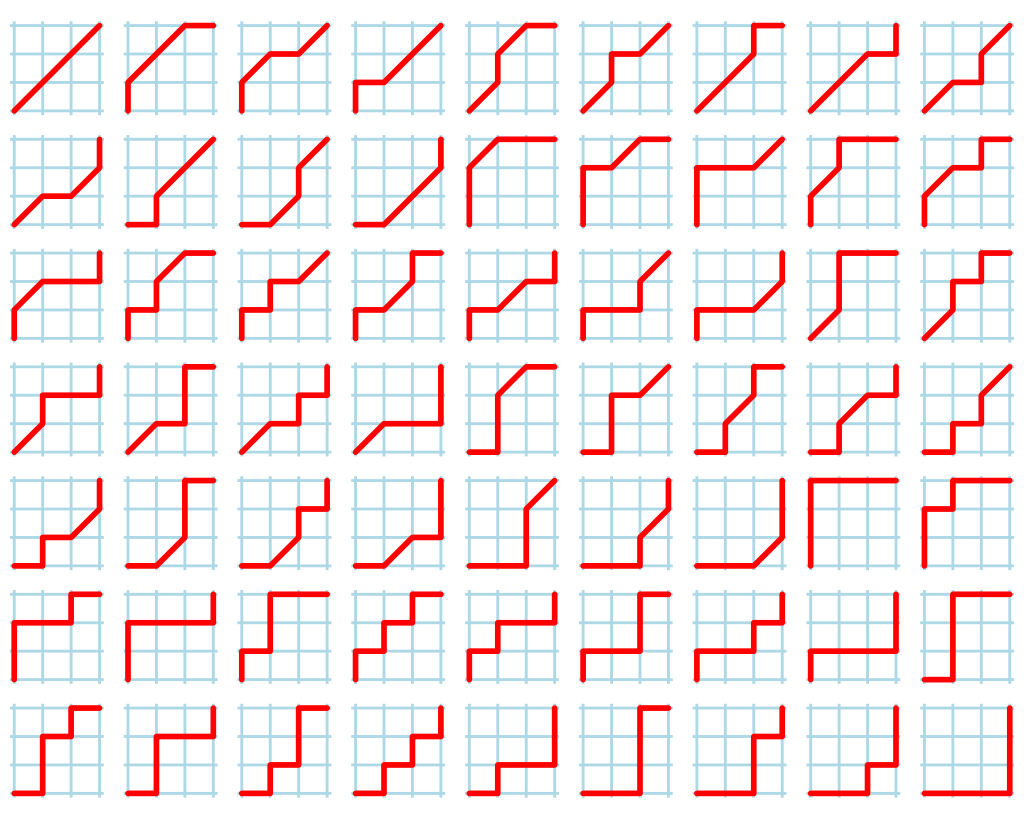
\includegraphics[width=10cm]{paths}\\
  Can you tell them how many different paths there are to their destination? 
  
  \subsection*{Input Format}
  The first and only line of input contains a single integer $n$.
  \subsection*{Output Format}
  The first and only line of your output must contain the number of different paths.
  \subsection*{Constraints}
  $0 \le n \le 100$
  \subsection*{Sample Input/Output}
  \begin{tabular}{ |l|l| } 
    \hline
    \textbf{Input} & \textbf{Output} \\
    {\lstinputlisting{./testCases/input/input02.txt}} & {\lstinputlisting{./testCases/output/output02.txt}} \\ % use {\lstinputlisting{./testCases/input/input00.txt}} & {\lstinputlisting{./testCases/output/output00.txt}}
    \hline
   \end{tabular}


  \section*{Solution}
  The number of paths from the southwest corner $(0, 0)$ of a rectangular grid to the northeast corner $(m, n)$, using only single steps north, northeast, or east is called a Delannoy Number $D(m,n)$. To find the answer, we must calculate $D(n,n)$.
  \subsection*{Solving the Problem}
  The recurrence relation for Delanoy Numbers where $m,n\neq0$ is
  $$D(m,n)=D(m-1,n)+D(m-1,n-1)+D(m,n-1)$$
  As $m$ and $n$ are equal, we calculate $D(n,n)=D(n-1,n)+D(n-1,n-1)+D(n,n-1)$.

	\section*{Sample Program}
	\lstinputlisting[language=Python]{sampleSolution.py}
	

\end{document}